\documentclass[free]{flammie}

\usepackage{ucs}

\usepackage{verbatim}
\usepackage{fancyvrb}

\usepackage{url}
\usepackage{graphicx}
\usepackage{linguex}

\usepackage{todonotes}

\setlength{\itemsep}{1pt}

\newcommand{\compresslist}{
\setlength{\itemsep}{1pt}
\setlength{\parskip}{0pt}
\setlength{\parsep}{0pt}
}








\newcommand\BibTeX{B{\sc ib}\TeX}
\newcommand\confname{ComputEL-5}
\newcommand\conforg{SIGEL}

\title{Reusing a Multi-lingual Setup to Bootstrap a Grammar Checker for a Very
Low Resource Language without Data\footnotepubrights{Published open access in
ACL workshop computel. \aclanthologypostprintdoi{2022.computel-1.19}}

\author{Inga Lill Sigga Mikkelsen\\
\\
  {\tt inga.l.mikkelsen@uit.no} \\\and{}
  Linda Wiechetek \\
  UiT Norgga árktalaš universitehta \\
  Divvun \\
  Norway  \\
   {\tt linda.wiechetek@uit.no} \\ \and{}
  Flammie A Pirinen \\
  \\
  {\tt flammie.pirinen@uit.no} \\}

\date{}

\begin{document}
\maketitle
\begin{abstract}
    Grammar checkers (GEC) are needed for digital language survival.  Very low
    resource languages like Lule Sámi with less than 3,000 speakers need to
    hurry to build these tools, but do not have the big corpus data that are
    required for the construction of machine learning tools.  We present a
    rule-based tool and a workflow where the work done for a related language
    can speed up the process. We use an existing grammar to infer rules for the
    new language, and we do not need a large gold corpus of annotated grammar
    errors, but a smaller corpus of regression tests is built while developing
    the tool.  We present a test case for Lule Sámi reusing resources from North
    Sámi, show how we achieve a categorisation of the most frequent errors, and
    present a preliminary evaluation of the system. We hope this serves as an
    inspiration for small languages that need advanced tools in a limited amount
    of time, but do not have big data.
\end{abstract}

\section{Introduction}

Language tools for very low resource languages are urgently needed to support
language maintenance, but also it takes a long time to develop them.  An
existing multilingual infrastructure and existing tools that can be reused can
speed up the process.  In this article, we describe the process of making a Lule
Sámi GEC together with a preliminary categorization of frequent Lule Sámi
errors.  Lule Sámi is on the lower end of lower resource language. It can
benefit from North Sámi which is closely related and has a well-functioning
grammar checker.


The reuse of existing knowledge is an important concept in effective development
of new grammar checkers in multilingual infrastructures.  With this work we
would like to set an example of how high-end complex NLP tools can be made, in
less time, by taking existing tools as a frame. The following tools were already
ready-made: an FST-based morphological analyser, a morpho-syntactic
disambiguator developed for correct text, and a multi-lingual infrastructure
that contains scripts to build the grammar checker (among other applications).
Our work took altogether 120 hours, (40 hours of meetings of two linguists (one
of them native speaker) and 40 hours of work of one native speaker linguist).

For related languages we can even reuse rules and sets (prenominal modifiers,
sentence barriers).  But for example, lexemes have to be translated.  This
article will show in detail what can be reused, and which factors need special
focus as they are language specific -- many times it is systematic homonymies,
and definitely idiosyncratic homonymies.  In addition, we will evaluate the Lule
Sámi grammar checker and point out future steps for improvement.

\section{Background}

\subsection{Language and resources}

Lule Sámi is spoken in northern Sweden and Norway, with an estimated 800--3,000
speakers~\cite{Sammallahti1998saami, Kuoljok2002barjas,
Svonni2008spraksituationen, Rydving2013words, moseley2010atlas}.  The Lule Sámi written
language was approved in 1983~\cite{Magga1994hvordan}.  The first Lule Sámi
spell checker was launched in 2007.  Lule Sámi is a morphologically complex
language, for more details see~\cite{Jussi2022}.

In 2013 the Lule Sámi gold corpus of writing errors was
built.\footnote{\url{https://github.com/giellalt/lang-smj/}} The gold corpus
consists of 32,202 words with 3,772 marked writing errors. The goal of this
error marked-up corpus was to test if the spellchecker corresponds to relevant
quality requirements, by running the spell checker on an error corpus, where
spelling errors were manually marked and corrected.  It was supposed to be
usable for testing grammar checkers with some processing, and therefore also
marked syntactic, morpho-syntactic and lexical errors. The texts gathered for
the gold corpus were written by native Lule Sámi speakers and had neither been
spellchecked nor proofread.

Speakers of Lule Sámi do not have a long written tradition, this amount of
errors in the gold corpus show that native speakers of Lule Sámi are in need of
tools helping them in the writing process. 1,774 of the errors in the gold
corpus are non-word errors (i.e.\ misspellings that result in a non-existent
form, non-word error, as opposed to real word errors where the misspelling
results in an existing `wrong' form), found by the spellchecker, the remaining
1,998 errors are morpho-syntactic, syntactic, word choice and formatting errors,
which only a grammar checker can detect and correct.  Lule Sámi is by UNESCO
classified as a severely endangered language.  For the (re)vitalisation of a
language, it is important that the language is actually being used. With a
(re)vitalisation perspective, a grammar checker for Lule Sámi will make it
easier for people to use Lule Sámi in writing, which will increase the use of
written Lule Sámi.

The marking and correcting of errors for the gold corpus is the first systematic
work on Lule Sámi writing errors. So far, this gold corpus has not been used to
analyse and describe error types characteristic for Lule Sámi. Our own
experiences from proofreading and from the work with North Sámi were therefore
the starting point for developing grammar rules.




\subsection{Framework}

The technological implementation of our grammar checker is based on
well-established technologies in the rule-based natural language processing:
finite-state automata for morphological
analysis~\cite{beesley2003finite,linden2013hFST} and constraint
grammar~\cite{karlsson1990constraint,bick2015cg} for syntactic and semantic as
well as other sentence-level processing.  The Lule Sámi has an existing
morphological analyser and lexicon publicly
available\footnote{\url{https://github.com/giellalt/lang-smj/}}, which were
originally imported from North Sámi with all rules and set specifications and
then adapted to Lule Sámi. \cite{Antonsen2010reusing}~report F-scores of 0.95
for part-of-speech (PoS) disambiguation, 0.88 for disambiguation of inflection
and derivation, and 0.86 for assignment of grammatical functions (syntax) for
the Lule Sámi analyser.

The system is built on a pipeline of modules: we process the input text with
morphological analysers and tokenisers to get annotated texts, then disambiguate
and then apply grammar rules on the disambiguated sentences, c.f.
Figure~\ref{fig:modules}.

\begin{figure*}
    \centering
    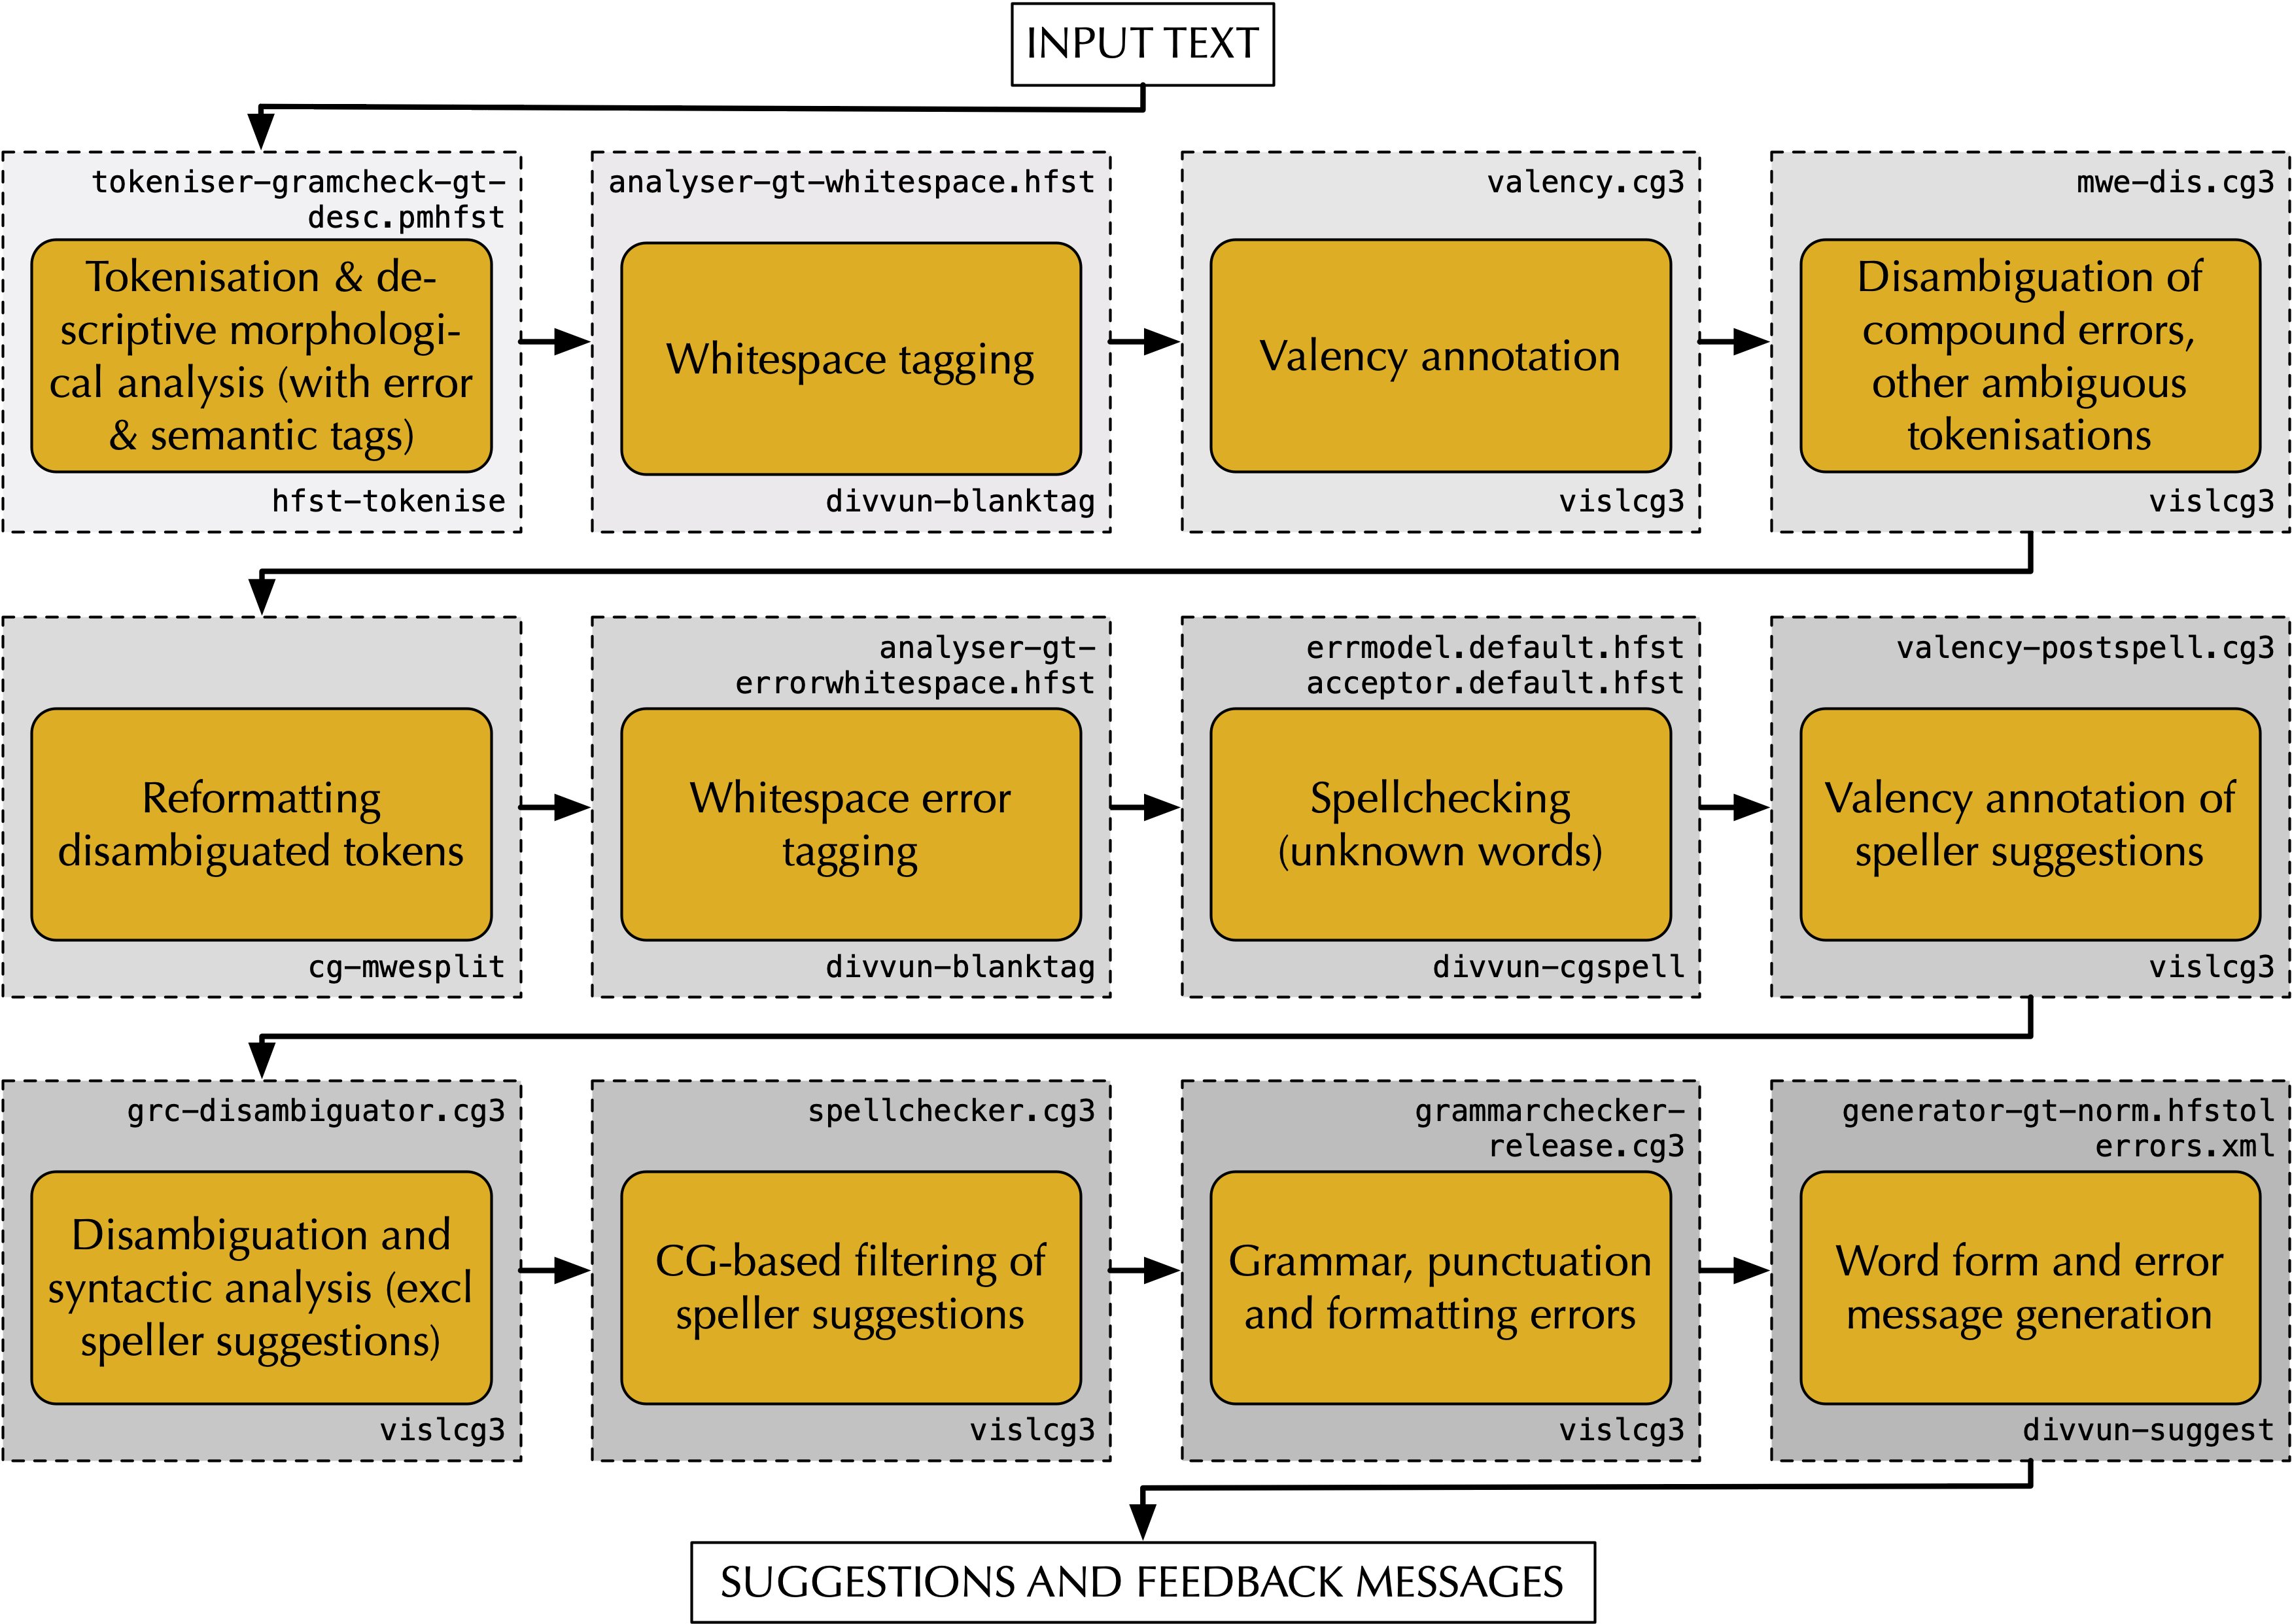
\includegraphics[width=.9\textwidth]{GramCheckLightFlow-08-2021.png.png}
    \caption{Structure of a grammar checker\label{fig:modules}}
\end{figure*}

It is noteworthy, that the system is part of a multilingual infrastructure
\textit{\href{https://github.com/giellalt}{GiellaLT}}, which includes numerous
languages --- 130 altogether.

The grammar checker takes input from the finite-state transducer (\textit{FST})
to a number of other modules, the core of which are several Constraint Grammar
modules for tokenisation disambiguation, morpho-syntactic disambiguation and a
module for error detection and correction. The full modular structure
(Figure~\ref{fig:modules}) is described in Wiechetek~\cite{Wiechetek2019many}.
We are using finite-state morphology~\cite{beesley2003finite} to model word
formation processes.

The technology behind our \textit{FSTs} is described in
Pirinen~\cite{Pirinen2014state}.  Constraint Grammar is a rule-based formalism for
writing disambiguation and syntactic annotation
grammars~\cite{Karlsson1990constraint,Karlsson1995constraint}.  In our work, we
use the free open source implementation VISLCG-3~\cite{bick2015cg}. All
components are compiled and built using the \textit{GiellaLT}
infrastructure~\cite{Moshagen-etal-2013-Building}.  The code and data for the
model is available for
download~\footnote{\url{https://github.com/giellalt/lang-smj/}}.

The syntactic context is specified in handwritten Constraint Grammar rules. The
ADD-rule below adds an error tag (identified by the tag
\texttt{\&real-negSg3-negSg2}) to the negation verb \textit{ij} `(to) not' as in
example~\ref{negsg3} if it is a 3rd person singular verb and to its left there
is a 2nd person singular pronoun in nominative case. The context condition
further specifies that there cannot be any tokens specifying a sentence barrier,
a subjunction, conjunction or a finite verb in between for the rule to apply.

\exg. Dån \textbf{ittjij} boade guossáj.\label{negsg3}\\
you \textsc{neg.past.sg3} come guest\textsc{.ill}\\
`You didn't visit.'

\begin{Verbatim}[frame=single,framerule=0.2mm,framesep=3mm,fontsize=\footnotesize,baselinestretch=1]
ADD (&real-negSg3-negSg2) TARGET ("ij")
IF (0 (Sg3))
(*-1 (Pron Nom Sg2)
BARRIER S-BOUNDARY OR
CS OR CC OR VFIN) ;
\end{Verbatim}

\section{Setup}

In this section, we answer the question of how to set up a grammar checker for a
new language in \textit{GiellaLT}. The resources we need are:

{\compresslist{}
\begin{enumerate}
    \item Word-based tools:
    \begin{itemize}
        \item a tokeniser / handling of multiword entities etc.
        \item an FST-based morphological analyser
        \item a spellchecker
\end{itemize}
    \item Sentence-based tools:
    \begin{itemize}
        \item a disambiguator (that can deal with erroneous input)
        \item a syntactic analyser
        \item a number of phonological or morpho-syntactic sets to categorise
            groups of words
        \item error detection/correction rules for a set of frequent errors
    \end{itemize}
    \item A set of frequent error types
    \item Regression tests (error-marked up test sentences)
\end{enumerate}
}



Unlike machine learning, this approach is not dependent on a large amount of
text data or a gold corpus. To develop a grammar checker, we only need several
test sentences containing the errors in
question.~\cite{wiechetek-etal-2021-fumbling} However, in the absence of a fully
error marked-up text corpus, finding frequent errors is a challenge.  We
therefore provide a scheme based on our experience with finding common errors
(for the North Sámi grammar checker) as a guideline for work on new languages.
This scheme serves any language, but our experience is based on morphologically
richer languages.

Error types can be divided into three main categories:
{\compresslist{}
\begin{enumerate}
    \item phonology-/typography-based errors
    \item (morpho-)syntactic errors
    \item writing convention-based errors
\end{enumerate}
}

Phonology-/typography-based errors can be based on diacritics, vowel/consonant
length, silent endings in certain contexts (\textit{-ij} pronounced
\textit{-i}), divergence pronunciation/writing and homophone words.

Writing/formatting conventions apply to compounding (one vs.\ several words,
hyphen), quotation marks, comma and punctuation in general.  Morpho-syntactic
and syntactic errors can be subdivided into verb-, NP-internal and VP-internal
issues.  NP-internal issues can be about prepositions and postpositions and
their case restrictions, adjective agreement /forms in attributive/predicative
positions, and relative pronoun agreement with its anaphora in number, gender
and animacy.

Verb internal issues concern the auxiliary construction, negation phrases (where
negation is expressed by  a verb) and other periphrastic verb constructions.

VP internal issues, on the other hand, are more global and concern subject-verb
agreement, subclauses formation, subcategorisation in general and case marking
of object/adverbial and word order.

In addition to that, the choice of error types will depend on efficiency as
well, that means which error types can rules generalize over, and which error
types are very word specific.  Very word specific work that cannot be
generalized may not be so efficient.

\subsection{Reuse of resources}

Reusing (particularly North Sámi) resources to create Lule Sámi tools goes back
as far as 2005, where the North Sámi descriptive morpho-syntactic
analyser/disambiguator was used to disambiguate Lule Sámi text and adapting work
started.  A disambiguator is a tool that resolves homonymy in a given syntactic
context, and is an essential tool in sentence-level text processing. This tool
was already available when we started our work. However, the initial goal of
sentence analysis is based on correct input. We therefore had to adapt the tool
to fit error input, e.g.\ by removing rules that were too strict and paying
closer attention to misspelled word forms that can be confused  with  correct
forms. In the course of time, other tools or modules have been copied over to
Lule Sámi and been reused with or without adaptations, thereby creating
lower-cost tools for Lule Sámi, cf.\ Table~\ref{reuse}.  Another tool that was
already available when we started to build our GEC was the Lule Sámi
morphological analyser. It had previously been constructed from scratch,
starting from a common template used in the \textit{GiellaLT} infrastructure.


\begin{table}[h]
    \centering
    \begin{tabular}{lll}
         \textbf{Tool} & \textbf{Reuse}  & \textbf{Adaption}\\
         \toprule
         \multicolumn{3}{c}{Analysis tools} \\
         \midrule
         \textbf{FST} & existing &  NONE \\
         \textbf{disambiguator} & from sme &  set specs \\
          &  & rules \\
         \textbf{tokeniser} & from sme &  NONE \\
         \midrule
         \multicolumn{3}{c}{Error detection/correction tools} \\
         \midrule
         \textbf{disambiguator} & from sme  & to fit err input \\
         \textbf{real w err rules} & NEW & --- \\
         \textbf{congr rules} & from sme & sets  \\
          & from sme & homonymies \\
         \midrule
         \multicolumn{3}{c}{Other} \\
         \midrule
         \textbf{regression tests} & NEW & --- \\
         \textbf{corpus mark-up} & from sme & applied to \\
                                 &          & smj text \\
         \bottomrule
         \end{tabular}
    \caption{Reuse of resources for Lule Sámi (sme= North Sámi, smj= Lule Sámi)\label{reuse}}
\end{table}

Based on our experience, we have found a following workflow to be very effective
in creating a new grammar checker: We use the normative morphological analyser
and a tokeniser with grammatical tokenisation disambiguation. This is relevant
when deciding if two words written apart have a syntactic relation or are simple
compound errors. In addition, there, we use a FST-based spellchecker.  The
descriptive disambiguator/syntactic analyser was first taken as it is to be
included in the Lule Sámi grammar checker. However, we found that the need for
adaptions was urgent, and we needed a separate version of it specifically for
potentially erroneous input. The difference to the descriptive disambiguator
lays in the objective. The descriptive disambiguator aims at a reduction of
homonymy (risking to some degree that correct analyses get lost). The grammar
checker disambiguator, on the other hand, needs disambiguation only to get an
idea of the sentence to find the error, but is dependent on finding
error-analyses even if they do not make sense in the context, so homonymy is not
to be reduced to a point where error readings disappear.  The descriptive
disambiguator is adapted on the fly, so basically every time testing runs into
problems, the respective rules are traced and either eliminated or adapted to
erroneous input.  In some cases, we also noticed general errors in the rules
that lead to an improvement of the descriptive disambiguator.






The error detection/correction module needed to be written from scratch at first
glance. However, at second glance, there are parts that could be reused as well.
Simple sets and lists were copied over from the Lule Sámi descriptive
disambiguator.  Semantic groupings of words developed in the process of North
Sámi grammar checking were directly copied over from the North Sámi grammar
checker, and lexical items translated to Lule Sámi as in the case of the
following set \textit{DOPPE} (the first of which is the North Sámi original, and
the second of which is the translated Lule Sámi one), which generalises over
static place-adverbs:

\begin{verbatim}
LIST DOPPE = "badjin" "bajil"
"dakko" "dá" "dákko" "dáppe" "dás"
"diekko" "dieppe" "do" "dokko"
"doppe" "duo" "duokko" "duoppe"
"olgun" ;

LIST DOPPE = "badjen" "dáppe"
"duoppe" "dåppe" "dággu" "daggu"
"duoggu" "dåggu" "dánna" "danna"
"duonna" "dånna" "dåhku" "duohku"
"ålggon" ;
\end{verbatim}





























As regards rules, the error types based on orthographic or phonetic similarity
needed to be written from scratch, as they differ in North Sámi and Lule Sámi,
as do possible contexts of errors that need to pay attention to homonymies.
Especially systematic homonymies are partly different to North Sámi. However,
some of them are the same in North Sámi and Lule Sámi, cf. Table
\ref{comparison}.  One of them is the homonymy between plural inessive (Lule
Sámi) /locative (North Sámi) and singular comitative nouns, and between singular
elative (Lule Sámi) /locative (North Sámi) and 3rd person singular possessive
accusative singular nouns.



\begin{table}[htb]
    \centering
    \begin{tabular}{lll}
         \textbf{Homonymy} & \textbf{Lule S.}  & \textbf{North S.}\\
         \toprule
         \multicolumn{3}{c}{\textbf{Verbs}} \\
         \midrule
         \textsc{Prs Pl3} --- \textsc{Prt Sg2} & sjaddi &  --- \\
         \textsc{Inf} --- \textsc{Prs Pl1} & --- &  šaddat \\
         \textsc{Prs Sg2} --- \textsc{Prs Sg3} & la &  --- \\
          \textsc{Prs Sg2} --- \textsc{Inf} & --- &  leat \\
                  \textsc{Prs ConNeg} &  &   \\
         \midrule
         \multicolumn{3}{c}{\textbf{Nouns}} \\
         \midrule
         \textsc{Pl Nom} --- \textsc{Sg Gen} & dile/mánno &  --- \\
         \textsc{Pl Ine} --- \textsc{Sg Com} & gielajn &  gielain \\
         \textsc{Sg Ela} ---  & girkus & girkkos \\
        \textsc{Sg Acc PxSg3} &  &  \\



         \bottomrule
         \end{tabular}
    \caption{Homonymies comparison  between Lule Sámi and North
    Sámi\label{comparison}}
\end{table}

Not all rules needed to be written from scratch, certain rule types were reused
from North Sámi.  Subject-verb agreement rules are well-suited to be copy-pasted
from North Sámi to Lule Sámi. With some tag adaptations, they were included into
the Lule Sámi grammar checker.





\subsection{Errors in Lule Sámi }

When working with the Lule Sámi grammar checker, we wanted to start with errors
made by high proficiency writers rather than language learners. That way we can
have a functioning grammar checker for texts with very few errors and introduce
more complex errors along the way. Texts written by second language learners or
students generally have more and other types of errors and more complex errors,
which will require a different grammar checker.

Typical errors of high proficiency writers happen when the written norm deviates
from the spoken dialectal variation. One example for that is the negation
paradigm, which in some dialects resembles the North Sámi paradigm rather than
the norm of written Lule Sámi.

In the Lule Sámi written norm, the negation verb is inflected for both person,
number and tense (present and past) followed by the main verb in connegative
form, which is always the same, whilst in North Sámi only person and number is
marked on the negation verb. Tense is marked on the main verb with two different
connegative forms, see Table~\ref{Negation}.



\begin{table}[h]
    \centering
    \begin{tabular}{llll}
    \multicolumn{2}{c}{Lule Sámi} & \multicolumn{2}{c}{North Sámi}\\
         \toprule
         \textbf{Present} & \textbf{Past} &  \textbf{Present} & \textbf{Past} \\
         \midrule
         \textit{iv vuolge} & {ittjiv vuolge} &  {in vuolgge} & {in vuolgán} \\
         \textit{i vuolge} & {ittji vuolge} &  {it vuolgge} & {it vuolgán} \\
         \textit{ij vuolge} & {ittjij vuolge} &  {ii vuolgge} & {ii vuolgán} \\
         \bottomrule
         \end{tabular}
    \caption{Negation comparison for `not leave'\label{Negation}}
\end{table}

There is no full consensus on the exact border between North Sámi and Lule
Sámi~\cite{Ylikoski2016future}, so in Lule Sámi text one can find variation regarding negation
that reflects dialectical variation. In Lule Sámi text both the North Sámi
negation system, as ex.~\ref{ex-aktak}, and a system with `double' past marking
on both the negation verb and with the main verb~\ref{ex-ittji} are used.

\exg. Aktak \textbf{ij} \textbf{vuolggám} nuorráj dan biejve.\label{ex-aktak}\\
someone not\textsc{.neg.pres.3sg} go\textsc{.pastp} sea\textsc{.sg.ill} that day
\\
`No one went on the sea that day.'

\exg. Gå ålgus vuolggi, de \textbf{ittji} \textbf{vuojnnám} åvvå
majdik.\label{ex-ittji}\\
when outside go\textsc{.past.2sg}, then not\textsc{.neg.past.2sg}
see\textsc{.pastp} all nothing \\
`When you went outside, you didn't see anything at all'

Most of the systematic morpho-syntactic errors made by high proficiency writers
reflect ongoing languages changes and might not even be corrected by a
proofreader. A grammar checker is a good way of making people aware of such
changes.

\textit{Soajttet} is a modal verb meaning `(to) maybe' and usually stands with
the infinitive form of the main verb. However, the present singular third-person
form \textit{soajttá} `(s/he) maybe' is by many writers being used as an adverb,
not as a modal verb, as example~\ref{ex-soajttá} shows. The modal auxiliary is
not followed by an infinitive as it should, but a finite verb in third-person
singular.

\exg. EU \textbf{soajttá} máhtti mijáv viehkedit.\label{ex-soajttá} \\
EU may\textsc{.pres.3sg} can\textsc{.pres.3pl} us help\textsc{.inf} \\
`EU might be able to help us'






Within noun phrases, writers frequently make agreement errors. According to the
norm the noun should be in singular with numerals and demonstratives agreeing in
case and number, according to~\cite{ylikoski2022lule} there is variation in the
contemporary language indicating that this agreement system is changing.  The
errors in the Divvun gold corpus show us that the change has gone further than
described in~\cite{ylikoski2022lule}, and numerals are handled in the same way as
attributive adjectives, see Table~\ref{Numerals}. Some writers seem to make use
of this ``new'' paradigm, as in ex.~\ref{ex-num}, while others seem to be
somewhere in between, as ex.~\ref{ex-num2} shows. In this last example, the case
of the numeral is correct, but the noun is in plural.

\exg. Alvos Státtáv máhtá vuojnnet gåjt \textbf{gietjav}
\textbf{báhppagieldajs}.\label{ex-num}\\
colossal Stáddá can see at.least seven\textsc{.num.nom.sg}
parish\textsc{.pl.ela}\\
`You can see the colossal Stáddá from at least seven parishes'

\exg.Suohkana juogeduvvin gietja sáme \textbf{rabdaguovlojda}.\label{ex-num2}\\
municipality divide seven\textsc{.num.ill.attr}  outskirt.area\textsc{.pl.ill.}
\\
`The municipalities got divided into seven  outskirt areas.'


\begin{table}[h]
    \centering
    \begin{small}
    \begin{tabular}{lll}
         \toprule
         \textit & \textbf{`(these) two cows'}\\
         \midrule
         \textit & \textbf{Norm} & \textbf{Systematical errors}\\
         \midrule
 Nom & (dá) guokta gusá & (dá) guokta gusá \\
 Gen & (dán) guovte gusá & (dáj) guokta gusáj  \\
 Acc & (dá) guokta gusá & (dájt) guokta gusájt  \\
 Ine & (dán) guovten gusán & (dájn) guokta gusájn  \\
 Ill & (dán) guovte gussaj & (dájda) guokta gusájda \\
 Ela & (dát) guovtet gusás & (dájs) guokta gusájs \\
 Com & (dájna) guovtijn gusájn & (dáj) guokta gusáj   \\
 \bottomrule
         \end{tabular}
         \end{small}
    \caption{NP with demonstrative pronouns and numerals\label{Numerals}}
\end{table}


Another noun phrase internal error is the use of and adjective in predicative
form in an attributive position, as example~\ref{ex-pred}. This is not a very
common error, but might be more frequent in texts written by second language
learners, since the predicative form is the one in dictionaries and the
adjective inflection system is one of the most complex area of the
morphology~\cite{ylikoski2022lule}. Along with this rule, we also made rules for
correcting errors where the attributive form of an adjective is used in a
predicative position.

\exg. Mij tjuovojma \textbf{roa\textipa{\ng}kok} bálggáv.\label{ex-pred}\\
We follow crooked\textsc{.sg.nom} path\textsc{.sg.acc}\\
`We followed a crooked path'








There are also agreement errors where relative pronouns fail to agree with their
anaphora in number, as in ex.~\ref{ex-rel5}, and not agreeing with its anaphora
in animacy, as in ex.~\ref{ex-rel6}.  A similar error regards the agreement of
reflexive pronouns with their anaphora in number.

\exg. Da sáme \textbf{gænna} ietjanisá ællim muorravuovdde\label{ex-rel5}\\
Those s\textsc{.pl.nom} who\textsc{.sg.ine} themselves have.not wood.forrest\\
`Those s without their own wood forrest'

\exg. Åhtsåp jådediddjev \textbf{mij}:\label{ex-rel6}\\
Search leader\textsc{.sg.acc} which\textsc{.nhum.sg.nom}\\
`We are looking for a leader who:'







Conditional mood is according to~\cite{ylikoski2022lule} largely missing in Lule
Sámi, and instead a periphrastic conditional consisting of the auxiliary lulu-
‘would’ and the infinitive is used. The conditional auxiliary \textit{lulu-} is
by some writers handled as if it is a separate verb with present and past tense,
not a mood, making errors like~\ref{ex-lulu} and the non-word
error~\ref{ex-lulu2}.

\exg.Vuorasulmutja \textbf{lulu} huvsov ja sujtov oadtjot.\label{ex-lulu}\\
old.people\textsc{.pl.nom} be\textsc{.cond.2sg} care and nursing get\textsc{.if}
\\
`Old people would get care and nursing '

\exg. \ldots{}sávvá ienebu \textbf{lulujin} kursajda
oassálasstet.\label{ex-lulu2}\\
\ldots{}wish more *would\textsc{.3pl} course attend.\\
`\ldots wishes more people would attend courses.'
















Another big group of errors are real-word errors. These are mostly based on
phonetic similarity between the confused forms. In this work, we focused on
general rules that are not limited to one single word, but rather forms that
apply to a group of lemmata. In Table~\ref{error-examples} the first error
(\textit{álgge}-\textit{álkke}) is an error limited only to  this specific word.
When in a hurry of building resources for  very low resource languages, one has
to make sure to work in an efficient way, and writing rules for correcting
specific words does not get us fast-forward. The rest of errors in
Table~\ref{error-examples} are errors being corrected by rules that generalise
over groups of words, or for the frequent negation auxiliary (function words are
more efficient).

\begin{table*}[h]
    \centering
    \begin{tabular}{p{4cm}p{4cm}p{6cm}}
         \textbf{Error} & \textbf{Correct form}  & \textbf{Type of error}\\
         \toprule
         \textbf{álgge} `beginner' & \textbf{álkke} `easy' &  Only for this
         single word \\
         \midrule
         \textbf{hábbmima} \textsc{NomAct Sg Gen} \textit{`the designing's'} &
         \textbf{hábbmijma} \textsc{Prt Pl1} `we designed' &  Systematic for all
         contracted -it verbs \\
         \midrule
         \textbf{bælosti} \textsc{Prs Pl3} `they defend' & \textbf{bælostij}
         \textsc{Prt Sg3} `s/he defended' & Systematic for all odd syllable -it
         verbs and auxiliary/copula \textit{liehket} \\
         \midrule
         \textbf{i/ittji} \textsc{Prs/Prt Sg2} & \textbf{ij/ittjij}
         \textsc{Prs/Prt Sg3} & Missing ``j'' for negation verbs Sg2 \\
           `you do/did not' & `s/he do/did not' &   \\
         \midrule
         \textbf{ij/ittjij} \textsc{Prs/Prt Sg3} & \textbf{i/ittji}
         \textsc{Prs/Prt Sg2} & Extra ``j'' for negation verbs Sg3\\
          `s/he do/did not' & `you do/did not'   \\
          \bottomrule
         \end{tabular}
    \caption{Real word errors comparison\label{error-examples}}
\end{table*}

The errors we have worked with in Table~\ref{error-examples} are all real word
errors with the ij-sound written `i', or the other way around, with `i' written
`ij'. We classified them as real word errors, even though some errors can also
be seen as agreement errors. High proficiency writers are typically not insecure
about agreement, but errors of this type can still happen when typing fast.
Another complicating factor is that the -i sound can also be written -ij. Odd
syllable nouns in illative case end in -ij, even though the pronouncation is not
-ij. `To the dog' is spelled \textit{bednagij} even though the actual pronounced
more like \textit{bednagi}. However, the spelling error \textit{bednagi} will be
picked up by the spell checker since it is a non-word.






















Both Lule Sámi and North Sámi verbs are inflected with three persons and three
numbers in past and present tense. The subject verb agreement rules were copied
from North Sámi to the Lule Sámi grammar checker.




\section{Evaluation}

The first version of the Lule Sámi grammar checker has 64 rules and 17 rule
types, three of which have a regression test of 50 or more test sentences.  We
also ran an initial evaluation of each regression test, and plan to run the
grammar checker on the error-marked up corpus of 32,202 words\footnote{Can be
found on GitHub:
\url{https://github.com/giellalt/lang-smj/tools/grammarcheckers}}.











Figure \ref{evaluation} shows an evaluation of three error types with a
sufficiently large regression tests. The other error types will be evaluated in
the final version of the paper. The rules for relative pronoun and
numeral/determiner agreement and for modal verb maybe-constructions give good
results for both precision and recall. Precision and recall of the modal verb
constructions are as good as 98\ The quality is measured using basic precision,
recall and $f_1$ scores, such that recall $R=\frac{t_p}{t_p+f_n}$, precision
$P=\frac{t_p}{t_p+f_p}$ and $f_1$ score as harmonic mean of the two: $F_1 = 2
\frac{P \times R}{P + R}$, where $t_p$ is a count of true positives, $f_p$ false
positives, $t_n$ true negatives and $f_n$ false negatives.

\begin{table}[htb]
    \centering \small
    \begin{tabular}{lrrr}
    \toprule
        \bf & \bf  Precision & \bf Recall & \bf $F_1$ \\
        \midrule
        Rel pronoun agreement & 81.43 & 83.82 & 82.61 \\
        Modal verb (`maybe') & 98.00 & 98.00 & 98.00 \\

        Num/det agreement & 74.14 & 67.19 & 70.49 \\

        \bottomrule
    \end{tabular}
    \caption{Performance  of the  grammar checker on three error types based on
    regression tests\label{evaluation}}
\end{table}












We also ran a test run of the automatic evaluation on the marked-up gold corpus
of Lule Sámi, to see if the grammar checker finds true errors and also to
improve the error mark-up of grammatical errors in the corpus, keeping in mind
that the corpus had been originally marked up for predominantly spelling errors.

A lot of errors found by the grammar checker are true positives. Many of them
were either not marked up or---more frequently---marked up with a different
scope. Since the start of marking up the corpora for spelling errors, the
mark-up guidelines have been developed further in connection with
\textit{GramDivvun}, the North Sámi grammar checker, and adapted to automatic
evaluation, where the grammar checker output is tested against the corpus
mark-up.

There are examples of when the grammar checker actually found grammatical errors
that the human proof-reader missed out.  Thirdly, there are examples where the
original marking is not consistent with the newer guidelines for how much the
scope of the error should be with regard to how much the grammar checker
actually marks up.  Example~\ref{msyn-mij-gut} is one of the cases where an
error in relative pronoun agreement has been identified correctly by the grammar
checker. This error type had a particularly high number of true positives in our
preliminary evaluation, showing that this is a frequent error type. Another very
frequent true positive that has not been adapted to current mark-up standards
regards numeral error types, as in~\ref{numeral-error}. The old mark-up would
have a bigger scope including context for the error, i.e. \textit{daj gålmmå
tiemáj birra>dan gålmå tiemá birra}. The current guidelines only mark up the
form that is to be corrected, meaning \textit{daj>dan}, \textit{gålmmå>gålmå}
and \textit{tiemáj>tiemá}  which are corrected in three steps and by three
separate rules.





\exg. Da ulmutja \textbf{ma} Hamsuna mielas li buorre ulmutja Hamsun gåvvi
buorak láhkáj.\label{msyn-mij-gut}\\
Those people\textsc{.pl.nom} which\textsc{.nhum.pl.nom} Hamsun mind is good
people Hamsun describe good way.\\
`Those people who, according to Hamsun, are good, he describes in a good manner'


\exg. Tjállagin li artihkkala \textbf{daj} \textbf{gålmmå} \textbf{tiemáj} birra
ma li ássje majna Árran la barggam \ldots\label{numeral-error}\\
Text is article these\textsc{.dem.pl.gen} three\textsc{.num.sg.nom} theme about
which is topics with Árran is work \ldots\\
`In the text there are articles about these three themes, which are topics Árran
has worked with'




















However, there are also several false positives, as in ex. \ref{falsepositive1},
where \textit{gålmmå} is not an error. The difficulty here is that the
subsequent noun form is homonymous between nominative and genitive, and the
numeral should have only been corrected if it was a genitive phrase.
False positives occurred specifically for this error type (in the case of
nominative/genitive nouns), showing that more work with the respective rules is
necessary to improve the performance of the grammar checker.


\exg. Ja gå Knut lij \textbf{gålmmå} jage vuoras de jåhtin Hábmelij, sadjáj
Hamsund.\label{falsepositive1}\\
And when Knut was three\textsc{.sg.nom} year\textsc{.sg.gen} old then move
Hábmel, place Hamsund\\
`And when Knut was three years old, they moved to Hábmel, to a place called
Hamsund'






In ex.~\ref{biejve}, on the other hand, the agreement error finding of the
grammar checker in \textit{álgij} `s/he started' and its correction to
\textit{álggin} `they started' is a false positive. This is based on there being
two subject candidates, because of singular nominative and plural genitive being
homonyms, (\textit{cuhppa}) and the other one plural (\textit{biejve}, which in
this sentence is singular genitive). The grammar checker confuses the first of
them for a subject and therefore wrongly adapts the verb to it.

\exg. Bierjjedagá sjnjilltjamáno 20. biejve \textbf{álgij} cuhppa, ja hiejtij
lávvodak iehkeda.\label{biejve}\\
Friday March 20. day\textsc{.sg.gen} begin\textsc{.past.sg3}
cup\textsc{.sg.nom}, and end saturday evening\\
`The cup started Friday on March 20 and ended Saturday evening'



















































Additionally, we tested the grammar checker on a manually proofread Lule Sámi
corpus used for a new text to speech (TTS) tool. The grammar checker did find
errors that the proofreader had missed and was therefore useful in a project
where we want the text to be perfect. Most of the responses from the grammar
checker on this corpus were however false positives, with the grammar checker
marking correct forms as errors. These `bad' results were in turn used to
improve and fine tune the grammar checker rules. We find this a very beneficial
way of working---using our tools to  double-check a proofread corpus, and at the
same time using the results of the corpus to improve our tools.

When running the grammar checker on a university level thesis, the grammar
checker found many real errors. It was interesting that some highly frequent
repeated errors were due to changes in the language norm.

The overall results show us that the grammar checker actually finds real errors,
but the main challenge with making it usable to users is to restrict the rules.
At this point there is too much noise with more false positives than true
positives.







\section{Conclusion}

We have shown that by using a related language grammar checker as a starting
point, we were able to create a basic level grammar checker for Lule Sámi,
categorise a fair amount of frequent error types and collect regression tests
for each of them in a reasonable amount of time (120 hours between two
linguists, one of them a native speaker).  The importance for language
revitalisation cannot be measured before integrating the tools in the respective
text processing programs for the language community to use. But we know from
experience with the spell checker, that the tools have a wide group of users,
and their importance can usually be felt in the number of complaints that are
sent when something is wrong with the distribution or other technical issues.

In the future, we want to offer a high-performance tool for the most common
error types to the Lule Sámi users. We aim to release a beta version together
with the commonly distributed spellchecker in 2022.\footnote{c.f.
\url{https://divvun.no/en/index.html}} From the developer side we aim at
regression tests of at least 100 examples per error type with at least 90 \


\section*{Acknowledgments}

We want to thank Børre Gaup for running the evaluation on the gold corpus and
helping with the technical side of error mark-up and automatic evaluation.

\bibliographystyle{unsrt}
\bibliography{computel3}

\appendix




\end{document}
